\documentclass[11pt,a4paper]{article}

% =====================
% Packages
% =====================
\usepackage[utf8]{inputenc}
\usepackage[T1]{fontenc}
\usepackage{amsmath,amsfonts,amssymb}
\usepackage{geometry}
\usepackage{graphicx}
\usepackage{booktabs}
\usepackage{pgfplots}
\usepackage{listings}
\pgfplotsset{compat=1.18}

\geometry{margin=2.5cm}

\lstset{basicstyle=\ttfamily\small, breaklines=true, frame=single}

% =====================
% Title
% =====================
\title{\textbf{Optimisation du calcul des zéros de $\zeta$ :\\ pourquoi le calcul va vite}}
\date{\small Auteur : hprzeta --- \today}

\begin{document}
\maketitle

\begin{abstract}
\noindent
Ce document explique le \textbf{raisonnement mathématique} derrière l'accélération du
calcul des zéros non triviaux de la fonction $\zeta$ de Riemann sur la droite critique.
L'enjeu est de passer d'un débit de l'ordre de $1$ zéro/seconde à $15$--$20$ zéros/seconde.
L'idée centrale est de séparer rigoureusement deux opérations de nature différente ---
la \emph{détection} et l'\emph{affinage} --- et d'appliquer à chacune l'outil adapté.
\end{abstract}

% =====================
\section{Introduction : deux opérations distinctes}
% =====================

Localiser un zéro de $\zeta$ sur la droite critique se décompose en deux étapes
de natures \textbf{très différentes} :

\begin{enumerate}
\item \textbf{Détection} --- déterminer qu'un zéro se trouve \emph{quelque part} dans un
intervalle, par exemple entre $t = 14.05$ et $t = 14.10$. Opération grossière.
\item \textbf{Affinage} --- déterminer sa position \emph{exacte},
$t = 14.134725141\ldots$, à $12$ décimales.
\end{enumerate}

Les deux utilisent la même fonction $Z(t)$, mais \textbf{pas de la même façon}.
Toute l'optimisation repose sur cette distinction : confondre les deux conduit à utiliser
partout l'outil le plus lent et le plus précis, ce qui est inutile pour la détection.

% =====================
\section{La fonction $Z$ de Hardy}
% =====================

On ne cherche pas les zéros de $\zeta$ directement : on passe par la fonction $Z$ de Hardy,

\[
Z(t) = \Re\left(e^{i\theta(t)}\,\zeta\left(\tfrac{1}{2}+it\right)\right),
\]

où $\theta(t)$ est la phase de Riemann--Siegel. Sa propriété décisive est que
\textbf{$Z(t)$ est réelle} pour $t$ réel, avec $|Z(t)| = \left|\zeta\left(\tfrac{1}{2}+it\right)\right|$.
On en déduit l'équivalence fondamentale :

\[
\zeta\left(\tfrac{1}{2}+it\right) = 0 \iff Z(t) = 0 .
\]

Chercher un zéro de $\zeta$ revient ainsi à chercher un \textbf{changement de signe}
d'une fonction réelle.

% =====================
\section{Étape 1 --- Détection : seul le signe compte}
% =====================

On balaie $t$ par petits pas. Un changement de signe de $Z$ entre deux points consécutifs
implique, par le théorème des valeurs intermédiaires ($Z$ continue), la présence d'un zéro :

\[
Z(14.05) = +1.1, \quad Z(14.10) = -0.3
\;\Longrightarrow\; \exists\, \gamma \in [14.05,\,14.10],\ Z(\gamma)=0 .
\]

Pour cette étape, \textbf{aucune haute précision n'est requise} : seul le signe importe.
Une évaluation vectorisée \texttt{Z\_batch()} (NumPy, voire GPU) calcule $Z$ sur tout un
tableau de $t$ en une opération, soit un gain d'environ $\times 50$ par rapport à des appels
séquentiels de \texttt{mpmath.siegelz}.

% =====================
\section{Formule de Riemann--Siegel et nombre de termes}
% =====================

L'évaluation de $Z(t)$ utilise la formule de Riemann--Siegel :

\[
Z(t) \approx 2\sum_{n=1}^{N}\frac{\cos\left(\theta(t)-t\log n\right)}{\sqrt{n}} + R(t),
\qquad
N = \left\lfloor \sqrt{\frac{t}{2\pi}} \right\rfloor .
\]

Le point clé : le nombre de termes $N$ \textbf{dépend de $t$}.

\begin{center}
\begin{tabular}{rcl}
\toprule
$t$ & $N=\lfloor\sqrt{t/2\pi}\rfloor$ & Précision interne RS \\
\midrule
$14$    & $1$  & imprécise ($\sim 10^{-2}$) \\
$300$   & $6$  & limite \\
$1000$  & $12$ & correcte \\
$10000$ & $39$ & très précise \\
\bottomrule
\end{tabular}
\end{center}

La croissance de $N$ en $\sqrt{t}$ est illustrée ci-dessous : pour les petits $t$, la somme
comporte trop peu de termes pour être fiable.

\begin{center}
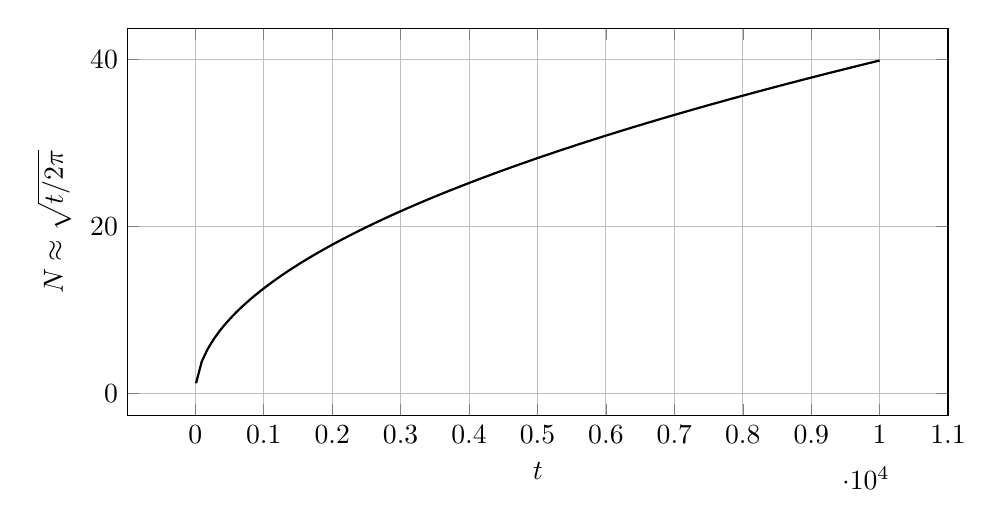
\begin{tikzpicture}
\begin{axis}[
xlabel={$t$},
ylabel={$N \approx \sqrt{t/2\pi}$},
grid=both,
width=12cm,
height=6.5cm,
domain=10:10000,
samples=120
]
\addplot[thick] {sqrt(x/(2*3.14159265))};
\end{axis}
\end{tikzpicture}
\end{center}

% =====================
\section{Seuil d'affinage : $t \geq 300$}
% =====================

L'affinage en C (module \texttt{illinois\_mpfr.so}) recalcule $Z$ via sa propre formule RS
interne. Il n'est fiable que lorsque $N$ est suffisant, c'est-à-dire pour $t \geq 300$
($N \geq 6$). En dessous, on bascule sur \texttt{mpmath} (\emph{fallback}), ce qui ne
concerne que :

\[
\#\{ \gamma_n : \gamma_n < 300 \} \approx 87 \quad \text{sur } 10\,142,
\qquad \text{soit } < 1\,\% .
\]

On conserve donc la vitesse du C sur $99\,\%$ des zéros.

% =====================
\section{Étape 2 --- Affinage : la méthode d'Illinois}
% =====================

Un zéro étant encadré dans $[a,b]$ avec $Z(a)Z(b)<0$, on trace la sécante reliant
$(a, Z(a))$ et $(b, Z(b))$ ; son intersection avec l'axe donne l'estimation :

\[
c = b - Z(b)\,\frac{b-a}{Z(b)-Z(a)} .
\]

On conserve le sous-intervalle qui encadre encore le zéro et on itère, resserrant
l'encadrement à chaque tour.

\paragraph{Pourquoi « Illinois ».}
La méthode brute (\emph{regula falsi}) peut voir une borne \textbf{stagner}, ralentissant
fortement la convergence. La correction d'Illinois : lorsqu'une borne stagne, on divise par
$2$ la valeur de $Z$ à cette borne, forçant la sécante à pivoter. On obtient une convergence
quasi quadratique \textbf{tout en garantissant l'encadrement} (aucune divergence possible).

\paragraph{Cas dégénéré.}
Si la détection place une borne quasi sur le zéro,
$|Z_b| \approx 6\times 10^{-14} \ll |Z_a| \approx 4\times 10^{-3}$, alors $c \approx b$
et Illinois stagne. La parade : retour immédiat de la borne quasi nulle, et en fin de boucle
retour de la meilleure borne (plus petit $|Z|$), jamais le milieu.

% =====================
\section{Parallélisme}
% =====================

Les intervalles à affiner sont \textbf{indépendants} : localiser $\gamma_{500}$ ne dépend pas
de $\gamma_{499}$. On répartit donc les intervalles sur les $4$ c\oe urs du processeur,
soit un gain d'environ $\times 4$.

\medskip
\noindent\textbf{Contrainte technique.} Le module C \texttt{.so} doit être chargé
\emph{après} le \texttt{fork()}, localement dans chaque \emph{worker} : les objets GMP/MPFR
ne se partagent pas proprement à travers un \texttt{fork()}.

% =====================
\section{Bilan de l'optimisation}
% =====================

\begin{center}
\begin{tabular}{lcc}
\toprule
Levier & Agit sur & Gain \\
\midrule
\texttt{Z\_batch()} vectorisé (NumPy/GPU) & détection & $\sim \times 50$ \\
\texttt{illinois\_mpfr.so} (C/libmpfr)    & affinage  & $\sim \times 39$ \\
$4$ \emph{workers} parallèles             & ensemble  & $\sim \times 4$ \\
\bottomrule
\end{tabular}
\end{center}

\noindent
Combinés, ces leviers font passer le débit de $\sim 1$ zéro/s (v5 séquentiel) à
$\sim 15$--$20$ zéros/s (v4.1). Un balayage complet jusqu'à $T=10\,000$ passe de plusieurs
heures à environ $10$--$15$ minutes.

\begin{center}
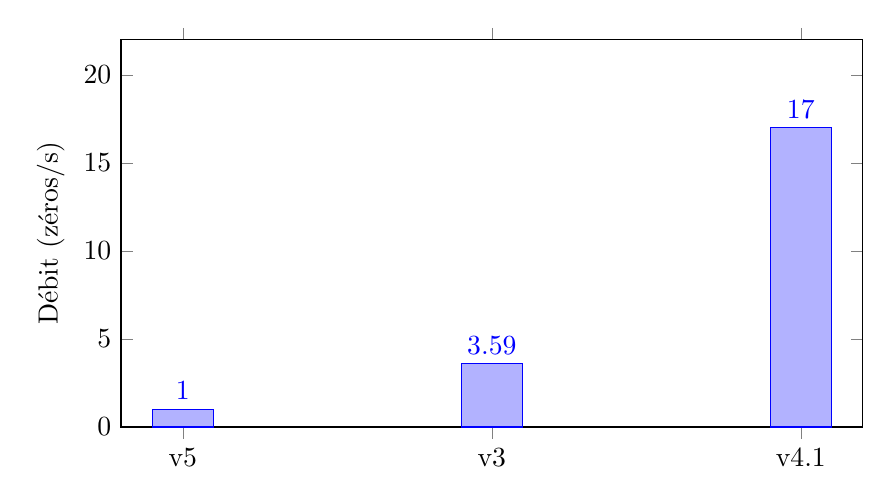
\begin{tikzpicture}
\begin{axis}[
ybar,
symbolic x coords={v5, v3, v4.1},
xtick=data,
ylabel={Débit (zéros/s)},
nodes near coords,
ymin=0, ymax=22,
width=11cm, height=6.5cm,
bar width=22pt
]
\addplot coordinates {(v5,1.0) (v3,3.59) (v4.1,17)};
\end{axis}
\end{tikzpicture}
\end{center}

% =====================
\section{Distinction expérimental / preuve}
% =====================

Ces méthodes \textbf{localisent numériquement} les zéros non triviaux de $\zeta(s)$ sur
$\Re(s)=\tfrac{1}{2}$. La validation de Turing--Backlund garantit la \textbf{complétude
numérique} (aucun zéro manqué) sur l'intervalle calculé. Ces résultats ne constituent
\textbf{pas une preuve} de l'Hypothèse de Riemann.

% =====================
\section{Annexe : code}
% =====================

Détection vectorisée (signe de $Z$) puis affinage par Illinois sur $t \geq 300$ :

\begin{lstlisting}
# Detection : signe de Z sur une grille (vectorise)
t_array = np.arange(t_debut, t_fin, step)
Z_vals  = Z_batch(t_array)                       # NumPy / GPU, ~x50
idx     = np.where(np.diff(np.sign(Z_vals)))[0]  # changements de signe

# Affinage : Illinois en C si t >= 300, sinon mpmath
for i in idx:
    a, b = t_array[i], t_array[i+1]
    if a >= 300.0:
        gamma = illinois_mpfr(a, b, tol)         # C / libmpfr, ~x39
    else:
        gamma = mpmath.findroot(mpmath.siegelz, (a + b) / 2)
\end{lstlisting}

\vfill
\noindent\rule{\textwidth}{0.4pt}\\
{\small Document créé le \today{} --- \texttt{Riemann\_Lab\_Optimisation.tex} ---
1 fichier source \LaTeX{} créé.}

\end{document}
